% system-model.tex

\documentclass[tikz]{standalone}
\usetikzlibrary{calc, positioning, arrows.meta}

\def\s{s}  % server
\def\b{bot} % literal string
\tikzset{seq/.style = {draw, circle, inner sep = 2pt, 
  scale = #1, left = 6pt}}

% csend: client sends operation to the server
\newcommand{\csend}[6]{
  % #1: client; #2: client pos; #3: server pos; #4: seq. number; #5: client state; #6: server state
  \draw[->] 
    ($(#1)!#2!(#1\b)$) 
    node[seq = 0.60, fill = red!40, label = {[label distance = -2pt]-90:\fbox{$#5$}}] 
    (#4) {#4} to 
    ($(\s)!#3!(\s\b)$) 
    node[seq = 0.50, label = {[label distance = 0pt]-90:\fbox{$#6$}}] 
    (server#4) {$#4$};
}

% ssend: the server sends operation to client 
\newcommand{\ssend}[5]{
  % #1: client; #2: server pos; #3: client pos; #4: seq. number; #5: client state
  \draw[->, dashed] 
    ($(\s)!#2!(\s\b)$) to ($(#1)!#3!(#1\b)$) 
    node[solid, seq = 0.50, fill = gray!40, label = {[label distance = 0pt]-90:\fbox{$#5$}}] 
    (cl#4) {$#4$};
}

\newcommand{\ins}[2]{$\textcolor{blue}{\textsc{Ins}(#1,#2)}$}
\newcommand{\del}[2]{$\textcolor{blue}{\textsc{Del}(#2)}$} 

\begin{document}
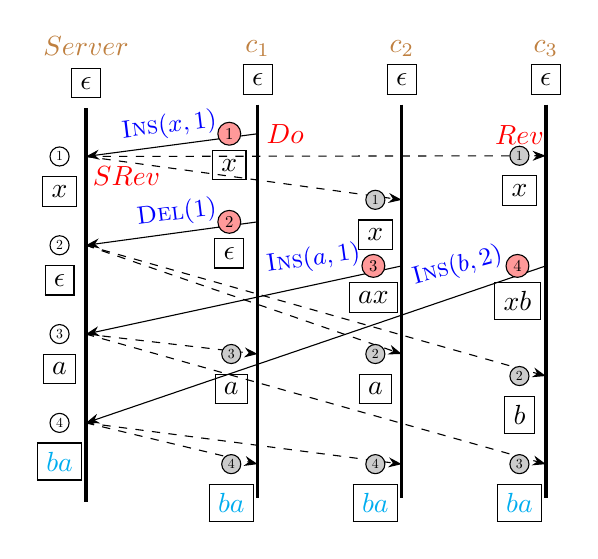
\begin{tikzpicture}[
    timeline/.style = {very thick}, >=Stealth, 
    op/.style = {font = \small, above left = -0.20cm and -0.10cm of #1, sloped},
    replica/.style = {align = center}]
  \node[replica] (\s) {\textcolor{brown}{$Server$} \\ \fbox{$\epsilon$}};
  \node[replica, right = 1.2cm of s] (c1) {$\textcolor{brown}{c_1}$ \\ \fbox{$\epsilon$}};
  \node[replica, right = 1.2cm of c1] (c2) {$\textcolor{brown}{c_2}$ \\ \fbox{$\epsilon$}};
  \node[replica, right = 1.2cm of c2] (c3) {$\textcolor{brown}{c_3}$ \\ \fbox{$\epsilon$}};

  \foreach \r/\rbot in {s/sbot, c1/c1bot, c2/c2bot, c3/c3bot} {
    \node[below = 5.0cm of \r] (\rbot) {};
    \draw[timeline] (\r) to (\rbot);
  }

  % send messages (ordered by positions at server)
  \csend{c1}{0.15}{0.20}{1}{x}{x}
  \node (o1) [op = {1}, rotate = 7] {\ins{x}{1}};
  \node (do) [right = 0.20cm of 1, red] {$Do$};
  \node (srev) [anchor = north, right = 5pt of server1, yshift = -7pt, red] {$SRev$};
  \ssend{c2}{0.20}{0.30}{1}{x}
  \ssend{c3}{0.20}{0.20}{1}{x}
  \node (rev) [anchor = north, above = 0pt of cl1, yshift = -3pt, red] {$Rev$};

  \csend{c1}{0.35}{0.40}{2}{\epsilon}{\epsilon}
  \node (o2) [op = {2}, rotate = 7] {\del{x}{1}};
  \ssend{c2}{0.40}{0.65}{2}{a}
  \ssend{c3}{0.40}{0.70}{2}{b}

  \csend{c2}{0.45}{0.60}{3}{ax}{a}
  \node (o3) [op = {3}, rotate = 8] {\ins{a}{1}};
  \ssend{c1}{0.60}{0.65}{3}{a}
  \ssend{c3}{0.60}{0.90}{3}{\textcolor{cyan}{ba}}

  \csend{c3}{0.45}{0.80}{4}{xb}{\textcolor{cyan}{ba}}
  \node (o4) [op = {4}, rotate = 15] {\ins{b}{2}};
  \ssend{c1}{0.80}{0.90}{4}{\textcolor{cyan}{ba}}
  \ssend{c2}{0.80}{0.90}{4}{\textcolor{cyan}{ba}}
\end{tikzpicture}
\end{document}
